\chapter{Background: Eclipse JDT and Jigsaw}\label{background2}

In order to construct structural generalizations describing the commonalities and differences between logged Java methods (LJMs), we need a concrete framework for constructing and manipulating abstract syntax trees (ASTs).  The Eclipse integrated development environment provides such a framework in its Java Development Tools (JDT) component.  The details of our implementation will depend on certain details of Eclipse JDT, so we describe those in Section~\ref{JDT}.

A framework exists for determining structural correspondences between AST nodes and measuring similarity between them, called Jigsaw \cite{2008:fse:cottrell}, which is described in Section~\ref{Jigsaw}. We build atop that work in order to create our anti-unifiers. Furthermore, an empirical study was conducted to assess how Jigsaw could effectively be used to address these issues.

\section{Eclipse JDT}\label{JDT}

The Eclipse Java Development Tools (JDT) framework provides APIs to access and manipulate Java source code via ASTs. An AST represents Java source code in a tree form, where the typed nodes represent instances of certain syntactic structures from the Java programming language.  Each node type (in general) takes a set of child nodes, also typed and with certain constraints on their properties.  Groups of children are named on the basis of the conceptual purpose of those groups; optional groups can be empty, which we can represent with the \NIL{} element. Thus, any Java source code can be represented as a tree of AST nodes. For example, the simple AST structure of two sample LJMs in Figures~\ref{ch3-ex1} an~\ref{ch3-ex2} is shown in Figure~\ref{fig:ast}

\begin{figure}[p]
\def\baselinestretch{1}
\begin{lstlisting}
public abstract class EBPlugin extends EditPlugin implements EBComponent {
    private Boolean seenWarning;

    protected EBPlugin() {
    }

    public void handleMessage(EBMessage message) {
        if(seenWarning) return;
        seenWarning = true;
        Log.log(Log.WARNING, this, getClassName() + " should extend EditPlugin not EBPlugin since it has an empty " + handleMessage());
    }
}
\end{lstlisting}
\caption{A Java class that uses a logging call. This will be referred to as Example 1.\label{ch3-ex1}}
\end{figure}

\begin{figure}[p]
\def\baselinestretch{1}
\begin{lstlisting}
public static class Wrapper implements ActionListener {
    private ActionContext context;
    private String actionName;

    public Wrapper(ActionContext context,  String actionName) {
        this.context = context;
        this.actionName = actionName;
    }

    public void actionPerformed(ActionEvent evt) {
        EditAction action = context.getAction(actionName);
        if(action == null) {
            Log.log(Log.ERROR, this, "Unknown action: " + actionName);
        }
        else
            context.invokeAction(evt, action);
    }
}
\end{lstlisting}
\caption{A Java class that uses a logging call. This will be referred to as Example 2.\label{ch3-ex2}}
\end{figure}

\begin{figure} [p]
  \centering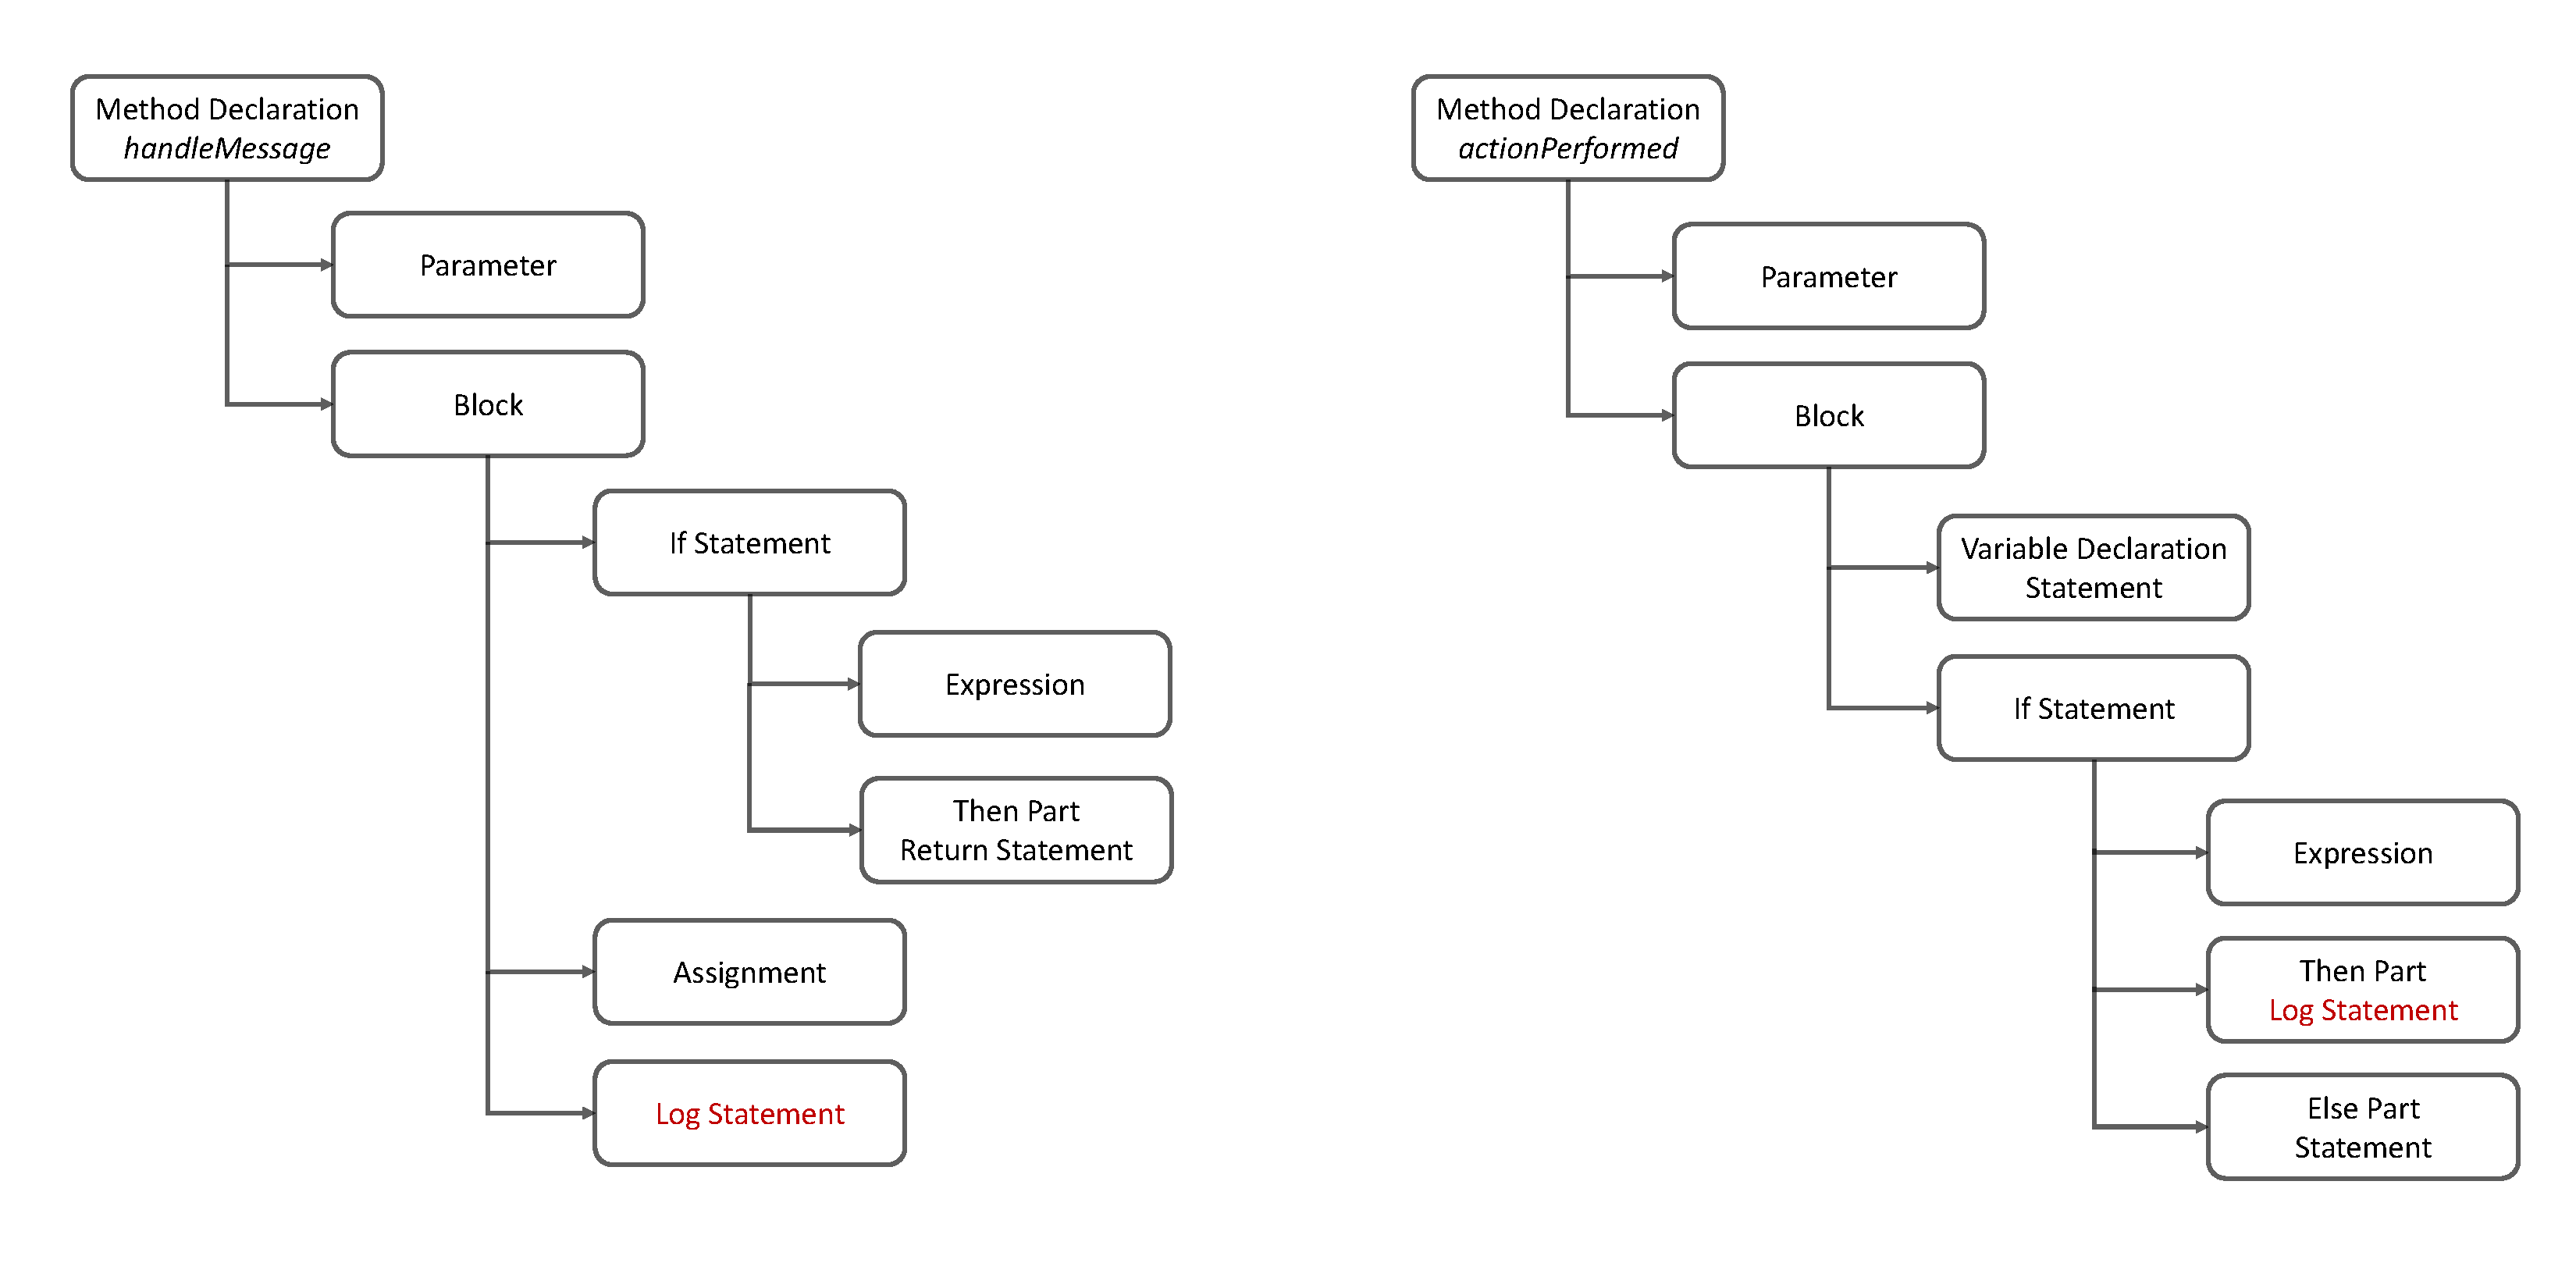
\includegraphics[width = \textwidth]{Drawing4/AST.pdf}
  \caption{Simple AST structure of examples in Figures~\ref{ch3-ex1} and~\ref{ch3-ex2}.}
  \label{fig:ast}
\end{figure}

In the JDT framework, structural properties of each AST node can be used to obtain specific information of the Java element that it represents. These properties are stored in a map data structure that associates each property to its value; this data is divided into three types:
\begin{itemize} [leftmargin=0.7in]
\item \textit{Simple structural properties:} These contain a simple value which has a primitive or simple type or a basic AST constant (e.g., identifier property of a name node whose value is a String).  For example, all the \textit{Identifier} nodes in Figure~\ref{fig:java-example-ast} fall in this case; each references an instance of \code{String} representing the string that constitutes the identifier.
\item \textit{Child structural properties:} These involve situations where the value is a single AST node (e.g., name property of a method declaration node).  For example, the \textit{ClassDeclaration} node in Figure~\ref{fig:java-example-ast} has a single child that represents its name as an \textit{Identifier} node; this would be a child structural property.
\item \textit{Child list structural properties}: These involve situations where the value is a list of child nodes.  For example, the \textit{ClassDeclaration} node in Figure~\ref{fig:java-example-ast} can possess multiple \textit{Modifier}s; these are recorded in the \textit{ClassDeclaration} as a child list structural property.
\end{itemize}

As an example, the ASTs of the logging calls at line~10 of Figure~\ref{ch3-ex1} and line~13 of Figure~\ref{ch3-ex2} can be represented respectively as:
\begin{itemize} [leftmargin=0.7in]
%\RW{These ASTs were messed up.  I fixed them according to what the code says.}
%\item \textit{expression(expression(Log), name(log), arguments(leftoperand(message), +, rightoperand(" is empty"), qualifier(Log), name(WARNING)))}
%\item \textit{expression(expression(Log), name(log), arguments(leftoperand(actionName),\\+, rightoperand("is an unknown action"), qualifier(Log), name(WARNING)))}
\item \textit{MethodCall}(\\
\hspace*{1em}\textit{QualifiedName}(\code{Log}, \textit{Identifier}(\code{log})),\\
\hspace*{1em}\textit{Arguments}(\\
\hspace*{2em}\textit{QualifiedName}(\code{Log}, \mbox{\textit{Identifier}(\code{WARNING})}),\\
\hspace*{2em}\textit{ThisExpression}(),\\
\hspace*{2em}\textit{AdditionExpression}(\\
\hspace*{3em}\textit{MethodInvocation}(\textit{Identifier}(\code{getClassName}), \textit{Arguments}()),\\
\hspace*{3em}\textit{StringLiteral}(\code{" should extend EditPlugin not EBPlugin since it has an empty "}),\\
\hspace*{3em}\textit{MethodInvocation}(\textit{Identifier}(\code{handleMessage}), \textit{Arguments}()))))\\
\item \textit{MethodInvocation}(\\
\hspace*{1em}\textit{QualifiedName}(\code{Log}, \textit{Identifier}(\code{log})),\\
\hspace*{1em}\textit{Arguments}(\\
\hspace*{2em}\textit{QualifiedName}(\code{Log}, \mbox{\textit{Identifier}(\code{ERROR})}),\\
\hspace*{2em}\textit{ThisExpression}(),\\
\hspace*{2em}\textit{AdditionExpression}(\\
\hspace*{3em}\textit{StringLiteral}(\code{"Unknown action: "}),\\
\hspace*{3em}\textit{Identifier}(\code{actionName}))))\\
\end{itemize}

\section{The Jigsaw framework}\label{Jigsaw}
The Jigsaw tool was developed by \citet{2008:fse:cottrell} to determine the structural correspondences between two Java source code fragments through the application of higher-order anti-unification modulo equational theories such that one fragment can be integrated to the other one for small-scale code reuse. Jigsaw could help determine potential candidate structural correspondences between AST nodes of LJMs by producing an augmented form of AST, called a \emph{correspondence AST} (CAST), where each node holds a list of candidate correspondence connections between the two structures, each implicitly representing an anti-unifier. Jigsaw also provides a measure of structural similarity to indicate how similar the nodes involved in each correspondence connection are. The Jigsaw similarity function relies on structural correspondence along with simple knowledge of semantic equivalences supported by the Java language specification. It returns a value in $[0, 1]$ where zero indicates complete lack of similarity and one indicates perfect similarity. In addition, several semantical heuristics are used to improve the accuracy of similarity measurement by allowing the comparison of AST nodes that are not syntactically identical but are semantically related to each other.

For example, the similarity between names of AST nodes is measured using a normalized computation based on the length of the longest common substring. The comparison of \code{int} and \code{long} types is another example, where an arbitrary value of 0.5 is defined as the similarity value as they are not syntactically identical but are semantically related. In addition, the Jigsaw framework also detects the structural correspondence between  \code{for}-, enhanced-\code{for}-, \code{while}-, and \code{do}-loop statements; and \code{if} and \code{switch} conditional statements. As an example, Figure~\ref{fig:meth-ast-1} shows the structural correspondence connections created by Jigsaw between the AST nodes of Examples 1 and 2 along with the similarity value for each correspondence connection.

\begin{figure} [H]
  \centering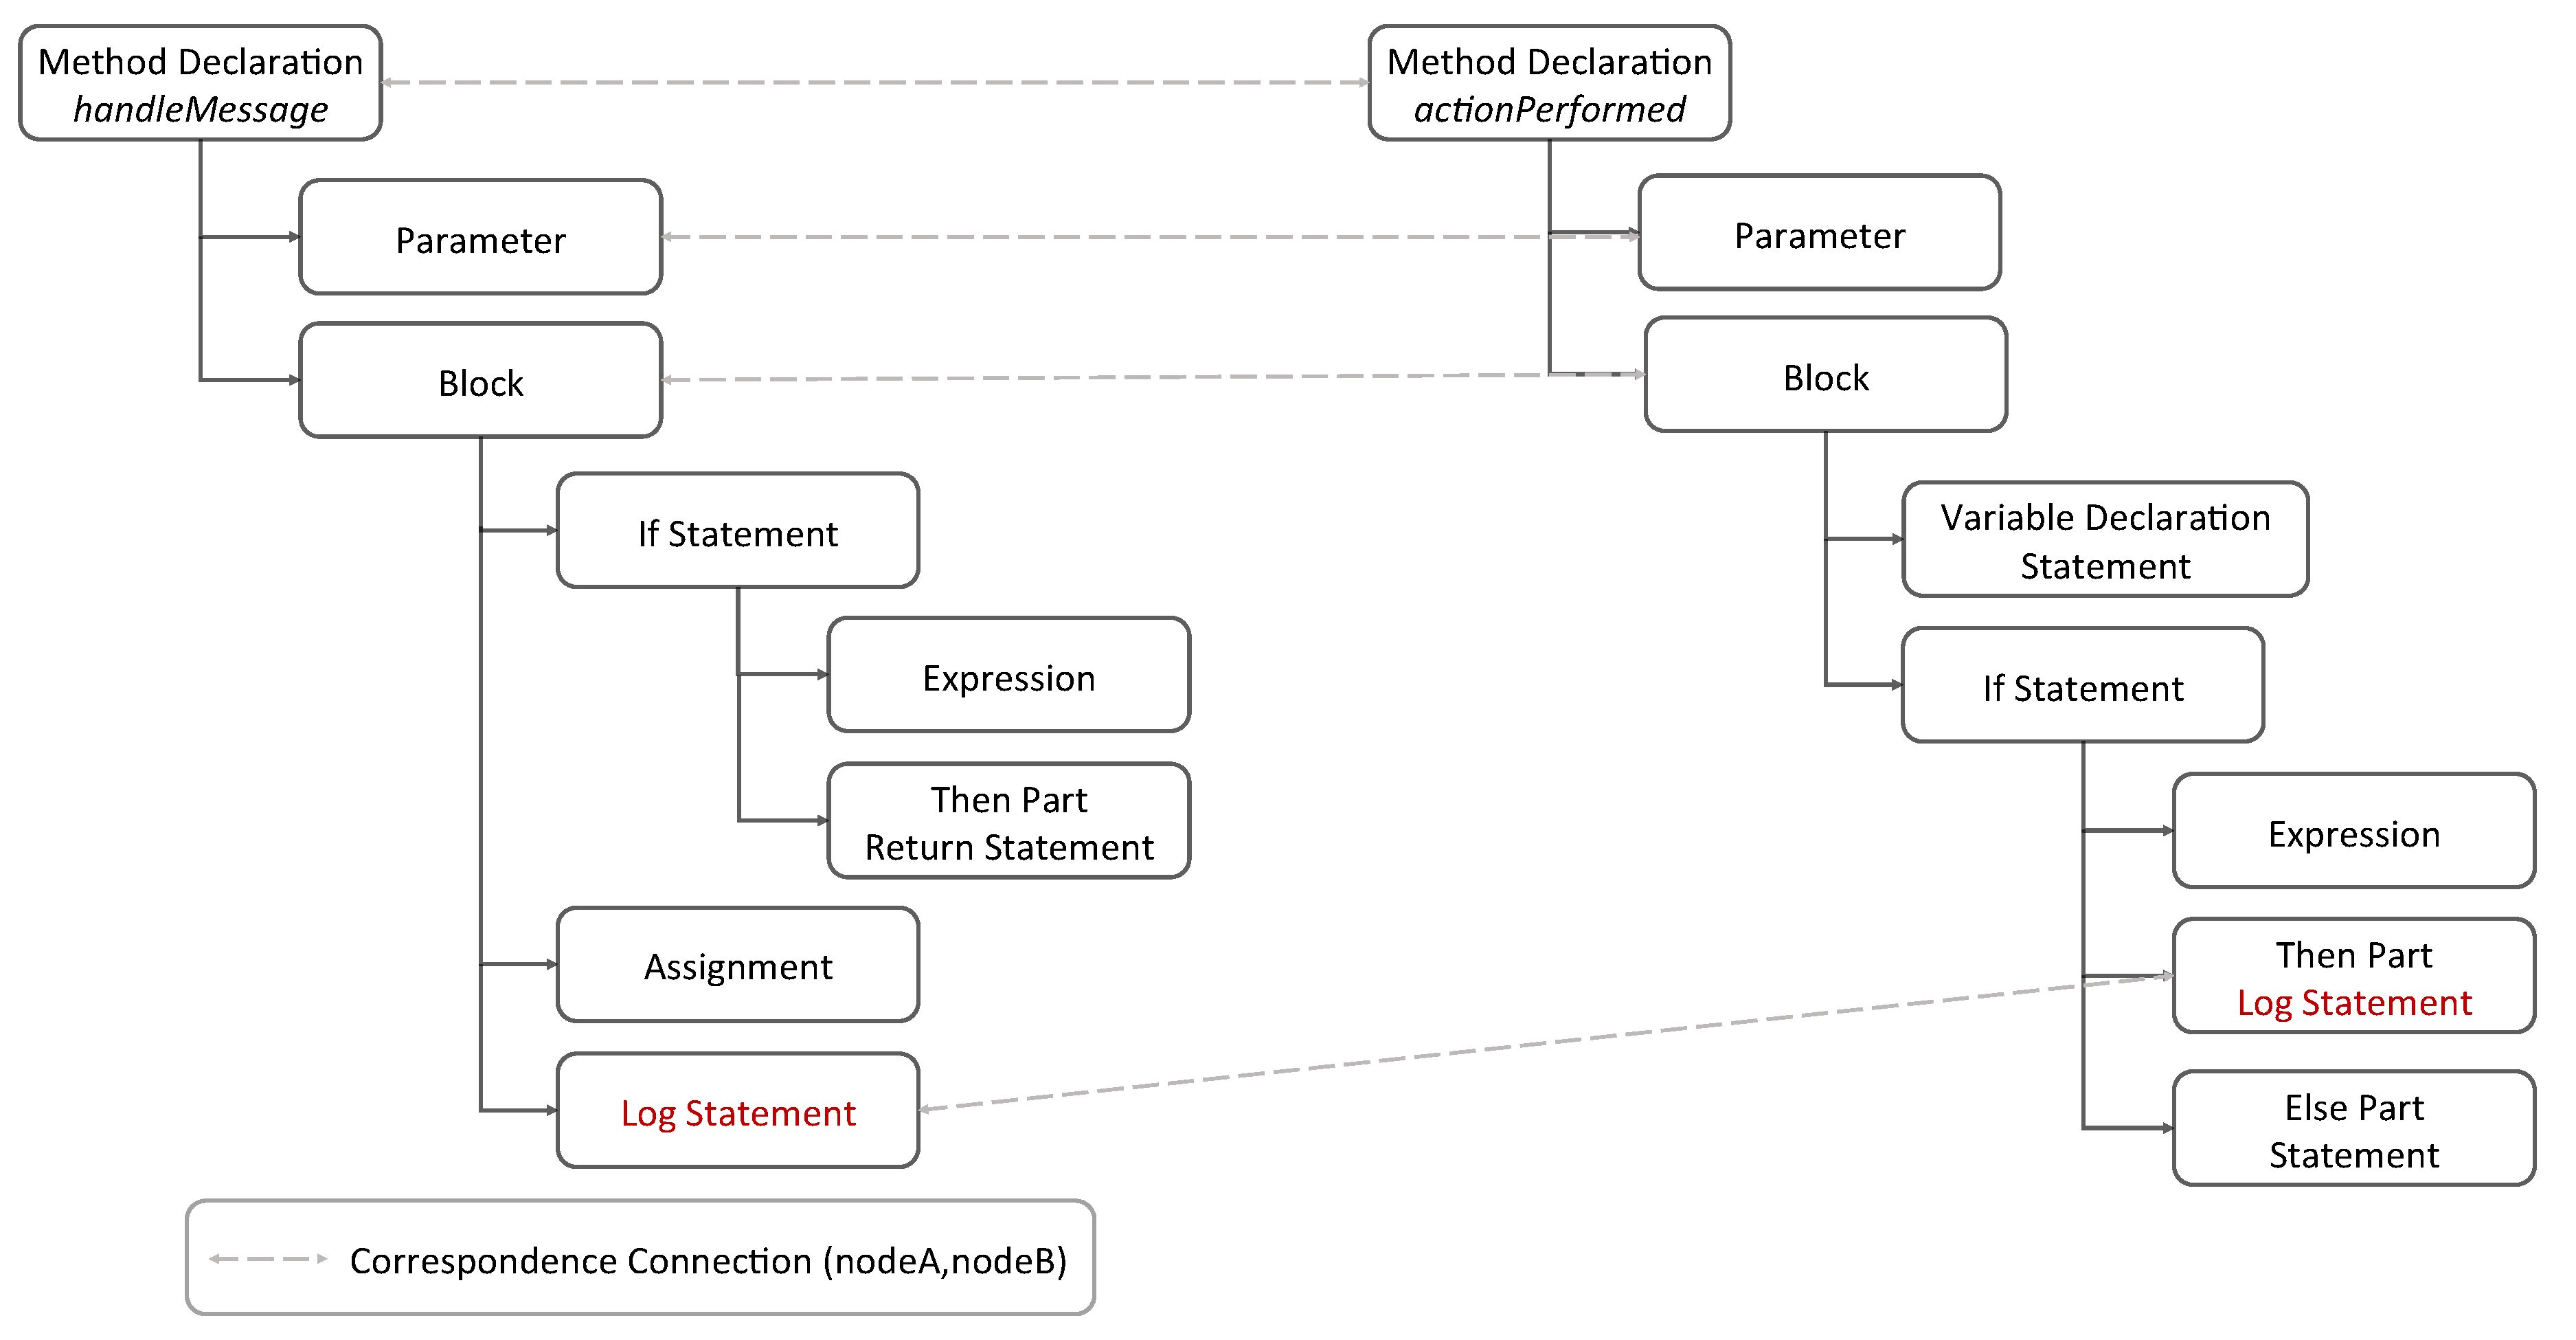
\includegraphics [width = \textwidth]{Drawing4/FirstCorr.pdf}
  \caption{Simple CAST structure of examples in Figures~\ref{ch3-ex1} and~\ref{ch3-ex2}. The links between AST nodes indicate structural correspondence connections created by the Jigsaw framework along with the similarity value.}
  \label{fig:meth-ast-1}
\end{figure}

However, the Jigsaw tool does not suffice to construct an anti-unifier that is the best fit to our application. In addition, the Jigsaw similarity function does not measure the similarity of two LJMs with a focus on logging calls, which is needed in our context. To address these issues, we should develop a greedy selection algorithm to approximate the best anti-unifier by determining the best correspondence for each node. In the following chapter, we will discuss our approach to construct structural generalizations and our implementation by means of the higher-order anti-unification modulo theories and the Jigsaw framework.


\section{An Assessment of Jigsaw}\label{jigsaw-assessment}

\RW{Describe here the procedure you used to select the examples, etc., how you tested Jigsaw, and what your findings were. At some point, you complained that Cottrell had not done something right ... do you have any evidence to demonstrate it?  How does this affect your work?  Such points can go in a discussion section towards the end of this chapter if they don't fit otherwise.  Full details of examples can go in an appendix; here, just describe enough so people can get the point.} 

\NZ{I think this experiment is not much about evaluating Jigsaw (The evaluation was conducted by Cottrell), but it is more about understanding what Jigsaw does and how to use it for my application . What I have mentioned was about detecting relevance links which is not related to my work. During my development, I added some statements to Jigsaw for the cases that was not covered in his work completely (e.g, Jigsaw did not detect the correspondence between inner type declarations of two nested type declarations when comparing the two upper type declarations } 

%chapter{Experimental Studies}  \label{studies}
%To evaluate our approach, we have implemented a tool, and conducted three empirical studies on a set of LJMs extracted from a real-world software system. In this section, we describe our experimental setup, present our studies, and discuss the results. 

We have conducted an experiment on a set of LJMs extracted from a real-world software system to assess how Jigsaw could effectively help us determine potential correspondences between AST nodes and measure similarity between them.
We implemented a plug-in to the Eclipse integrated development environment (IDE), which uses the \name{JDT} framework to extract ASTs of a pair of LJMs and applies the \name{Jigsaw} framework to generate correspondence connections between AST nodes. 

%the correspondence tool as
%\subsubsection{Experimental Setup}  \label{study1_setup}
\subsubsection{Setup}  \label{study1_setup}
%Our tool is a plug-in to the Eclipse integrated development environment (IDE) that implements our algorithm. The tool consists of three main components: a correspondence tool, an antiunifier-building tool, and a clustering tool. The correspondence tool inputs a pair of LJMs, uses the Jigsaw framework to determine potential correspondences between their AST nodes, and outputs the generated CASTs and the Jigsaw similarity between them. The antiunifier-building tool inputs a pair of LJMs, applies our anti-unification algorithm to construct an anti-unifier with a special attention to logging calls, and outputs the detailed view of anti-unifier and similarity measure (as described in Section~\ref{meth-antiUnifier}). The clustering tool inputs a set of LJMs, applies a hierarchical clustering algorithm to classify them based on the similarity measurement, and outputs the detailed view of the generated anti-unifier for each cluster (as described in Section~\ref{meth-clustering}). 
% figure of architecture?

As a subject for our study, we used \name{jEdit}, a programmer’s text editor tool written in Java programming language. We chose this subject because it is a real program that has been used constantly by many developers, and it employs real usage of logging calls. Our tool extracts all LJMs within the source code of this program. However, a subset of them was selected containing 9 LJMs that showed varying levels of similarity on manual examination, and it has been used as a test suite throughout this study (see Table~\ref{table:ljms}). The org.gjt.sp.jedit.EditBus.send(...) method contains two logging calls. To handle this case we split it into two cases: case 3 contained the first logging call while the second one was removed; case 4 contained only the second logging call. We will describe our approach for LJMs containing multiple logging calls in details in Section~\ref{meth-multipleLogs}. The last three LJMs were manually modified by adding some statements for the sake of dealing with important cases that we otherwise would have missed testing. Case 8 simulates the addition of an \code{if- }statement that formed a nested \code{if- }statement enclosing a logging call. Cases 9 and 10 simulate the addition of statements to improve the test coverage. 


\begin{figure} [H]
  \centering
  \begin{tabular}{|c|l|c|}
    \hline
    Case & Logged Java methods & Size(LOC)\\
    \hline
    1& org.gjt.sp.jedit.PluginJAR.generateCache() &104\\   
   \hline
    2& org.gjt.sp.jedit.MiscUtilities.isSupportedEncoding(...) &9\\   
   \hline
    3& org.gjt.sp.jedit.EditBus.send(...) &14\\   
   \hline
    4& org.gjt.sp.jedit.EditBus.send(...)* &14\\   
   \hline
    5& org.gjt.sp.jedit.EditAction.Wrapper.actionPerformed(...) &5\\   
   \hline
    6& org.gjt.sp.jedit.EBPlugin.handleMessage(...) &6\\   
   \hline
    7& org.gjt.sp.jedit.BufferHistory.RecentHandler.doctypeDecl(...) &3\\   
   \hline
    8& org.gjt.sp.jedit.JARClassLoader.loadClass(...) &32\\   
   \hline
    9& org.gjt.sp.jedit.io.VFS.DirectoryEntry.RootsEntry.rootEntry(...) &36\\   
   \hline
    10& org.gjt.sp.jedit.ServiceManager.loadServices(...) &20\\   
    \hline
  \end{tabular}
  \caption{Logged Java methods used as our test suite; all are contained in the \name{org.gjt.sp.jedit} package.}
  \label{table:ljms}
\end{figure}


%\subsubsection{Setup}  \label{study1-setup}
Our tool was used to compare LJMs of our test suite in a pairwise manner (55 test cases in total, including self-comparisons) and to produce the CASTs of each pair. The Jigsaw similarity was also measured for each of these test cases.
We examined the generated CASTs of these test cases and selected a subset of 4 cases with various levels of correspondences as depicted in the Table~\ref{jigsaw_4_test_cases}. Case 1 contains the comparison of a Java element with itself. Case 2 contains the comparison of two Java elements that are both syntactically and semantically dissimilar.  Case 3 contains the correspondence between two Java elements that are syntactically dissimilar but are semantically relevant. Case 4 contains the comparison of a logging call with another Java element that is not logging call but is syntactically relevant.

\subsubsection{Results}  \label{study1-results}
The results of the pairwise comparison between LJMs of the test suite is visualized in Figure~\ref{fig:jigsaw_graph}. As it is shown, the Jigsaw similarity for all self-comparisons is 1, while  the level of Jigsaw similarity is different for pairs containing distinct LJMs as our manual examination.

\begin{figure} [H]
  \centering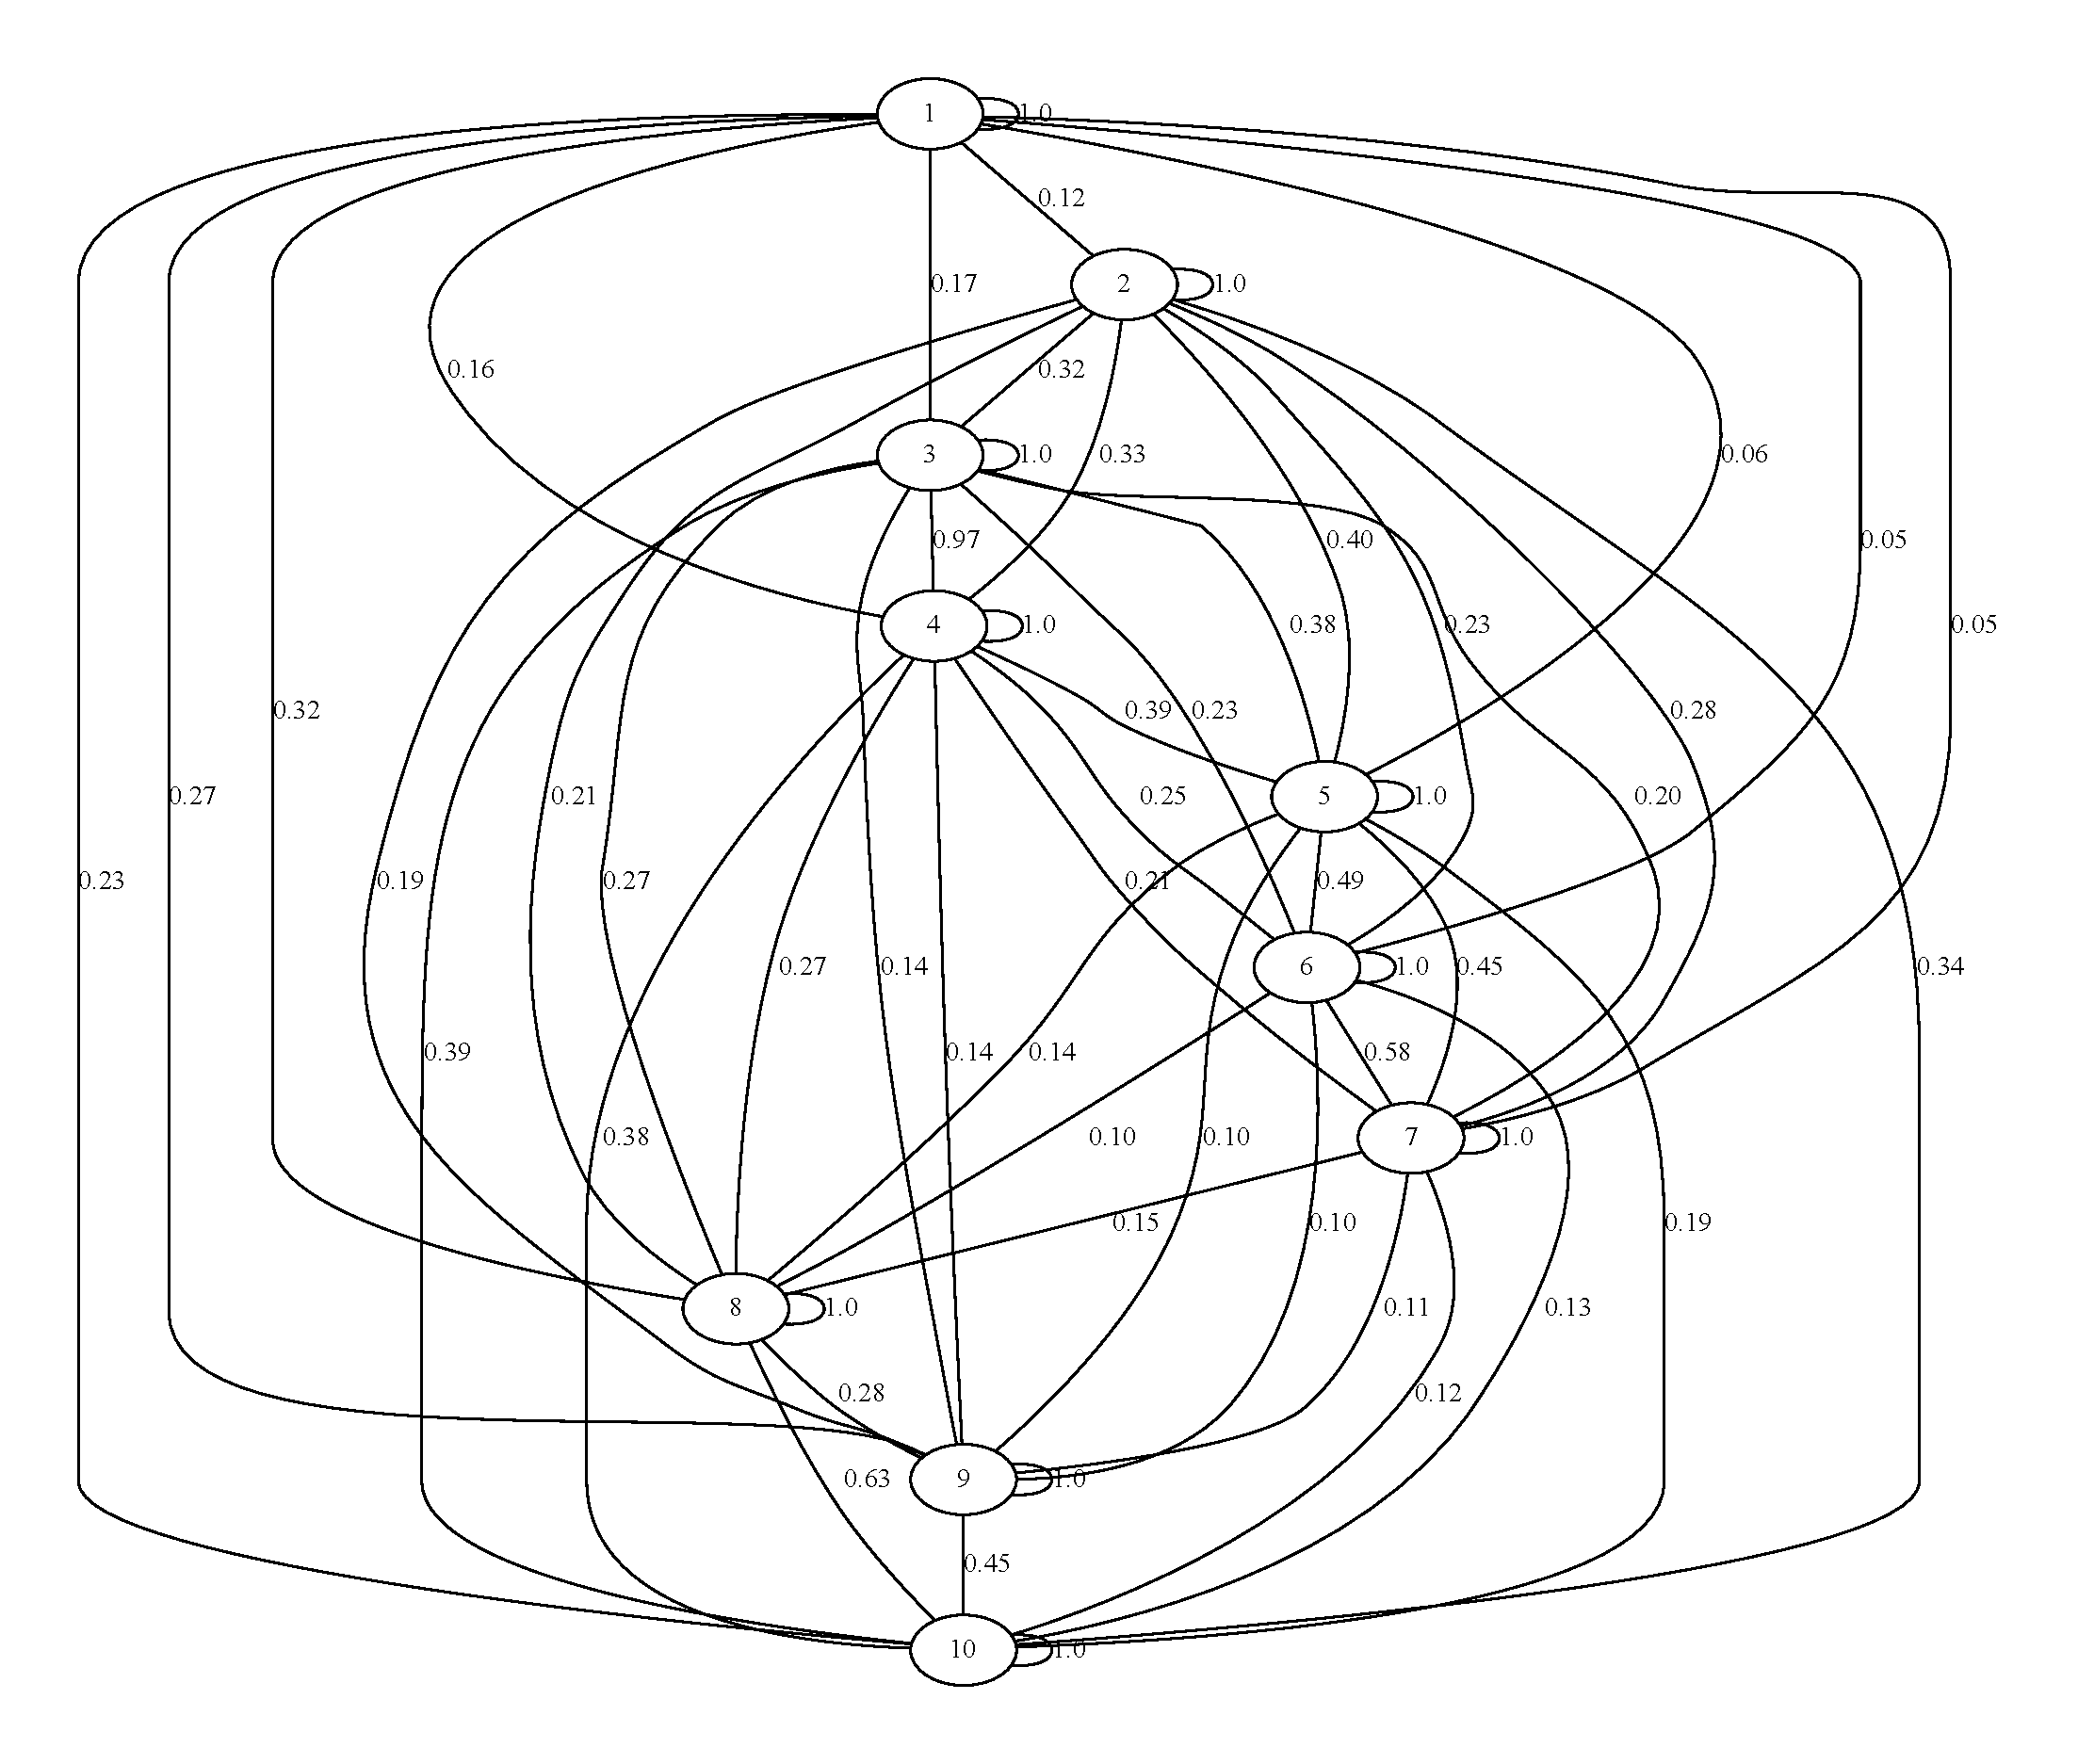
\includegraphics [width = \textwidth]{graphviz/jigsaw.pdf}
  \caption{A similarity graph representing pairwise Jigsaw similarities between LJMs shown in Table~\ref{table:ljms}.}
  \label{fig:jigsaw_graph}
\end{figure}


The analysis of the 4 test cases is shown in Table~\ref{jigsaw_4_test_cases}. Test Case 1 shows that a Java element that is compared with itself has a Jigsaw similarity of 1. Test Case 2 indicates that no correspondence connection is created when a Java element is compared with another Java element that is utterly dissimilar. Test Case 3 indicates that the similarity between a \code{for-} statement and a \code{while-} statement is non-zero, and that Jigsaw is able to detect semantic correspondences between Java elements. Test Case 4 shows that a logging call has non-zero similarity with another Java element that is not a logging call but is syntactically relevant. This case will be handled via the removal of this kind of correspondence connection, as will be described in Section~\ref{meth-constraints}. 

\begin{figure}
  \centering
  \begin{tabular}{|c|l|c|}
    \hline
    \shortstack{Test\\case} & Java source code fragment & \shortstack{Jigsaw\\similarity}\\
    \hline
    
    \multirow{2}{*}{{1}}&Log.log(Log.WARNING,this,"Unknown action: " + actionName);& \multirow{2}{*}{1}\\
    \cline{2-2}
                         &Log.log(Log.WARNING,this,"Unknown action: " + actionName);\\
    \hline
    
       \multirow{2}{*}{2}&return entry& \multirow{2}{*}{\shortstack{No\\correspondence \\connection}}\\
    \cline{2-2}
       &int i=0;\\
    \hline
  
    
 \multirow{2}{*}{3}&
 for (int i=0; i < comps.length; i++) {...} \\
  

    \cline{2-2}
      & 
while (entries.hasMoreElements())  { ...}    
      \\
    \hline    
    
    \multirow{2}{*}{4}&Log.log(Log.WARNING,this,"Unknown action: " + actionName);& \multirow{2}{*}{0.33}\\
    \cline{2-2}
      &EditBus.removeFromBus(this);\\
    \hline
    
  \end{tabular}
  \caption{Results from examining the Jigsaw similarity for 4 sample Java source code fragment pairs.}
  \label{jigsaw_4_test_cases}
\end{figure}
 


\section{Summary}  \label{summary}
We described Eclipse JDT as a concrete framework that can be used  to manipulate ASTs of a source code written in the Java programming language. We also introduced Jigsaw, an existing framework for determining structural correspondences between AST nodes and measuring similarity between them. Furthermore, we assess the Jigsaw functionality to address our problem through an empirical study on a set of LJMs selected from a real- world software system.

%In this chapter, we described anti-unification as a technique to construct a common generalization of two given terms. We have also introduced an extended form of anti-unification, which is called higher-order anti-unification modulo theories, where a set of equivalence equations can be applied on higher-order extended structures to incorporate background knowledge. In addition, we provided a brief description of AST that maps Java source code in a tree structure form, and why an extended form of it, named AUAST, is required to create higher-order structures specific to our problem context. Finally, we discuss the Jigsaw framework and how it could assist us in determining the potential structural correspondences.